% Generated by tools/paper/render.py from main_text.py; edit the source there, not this file.
\section{Methods}

\subsection{Overview}

sporos is implemented in Mojo \citep{Mojo}, which compiles through MLIR \citep{Lattner2021} to native code and exposes SIMD vectors as first-class types. Input may be FASTA or FASTQ, plain, gzip- or BGZF-compressed, with BGZF blocks decompressed in parallel. Bases are stored as 2-bit codes, one per byte, with a fifth code for other symbols. Three engines compute the seeds (Fig.~\ref{fig:overview}); all are multithreaded with POSIX threads and exposed through a Mojo API, C and Python bindings and a command-line tool that writes MUMmer's MEM format and \texttt{bwa fastmap}'s SMEM format.

% Generated by tools/paper/render.py from main_text.py; edit the source there, not this file.
\begin{figure*}[t]
\centering
\resizebox{\textwidth}{!}{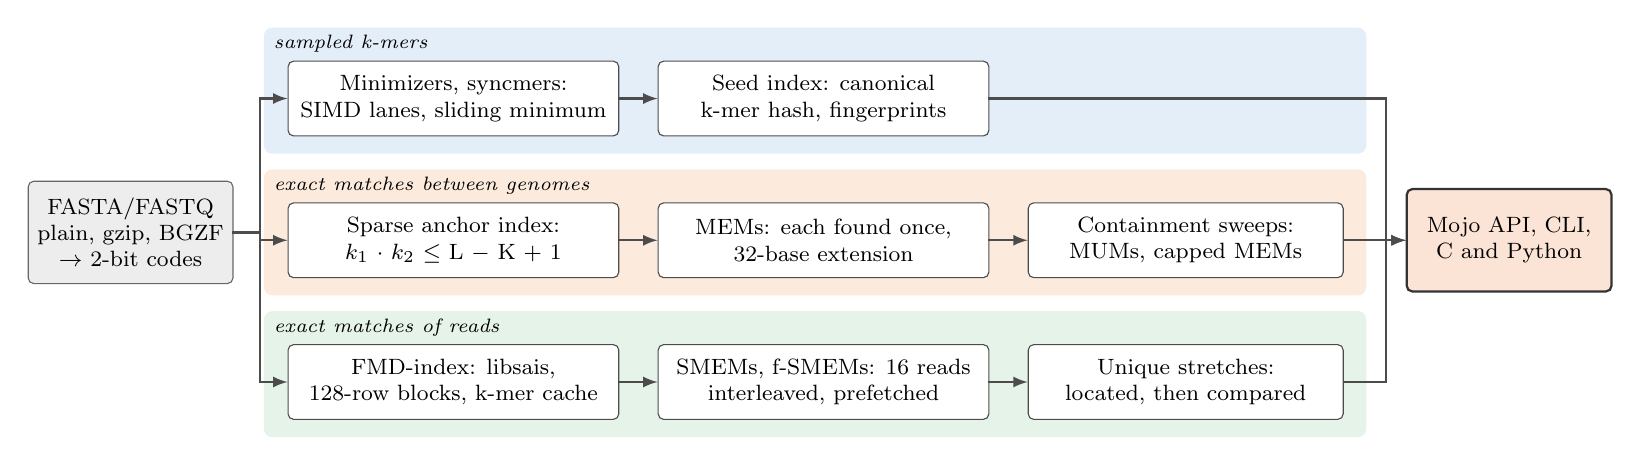
\begin{tikzpicture}
\fill[fill={rgb,255:red,227;green,238;blue,249}, rounded corners=3pt] (3.0,3.55) rectangle (17.0,5.15);\node[anchor=north west, font=\scriptsize\itshape, inner sep=2pt] at (3.05,5.130000000000001) {sampled k-mers};
\fill[fill={rgb,255:red,252;green,235;blue,221}, rounded corners=3pt] (3.0,1.75) rectangle (17.0,3.35);\node[anchor=north west, font=\scriptsize\itshape, inner sep=2pt] at (3.05,3.33) {exact matches between genomes};
\fill[fill={rgb,255:red,229;green,243;blue,232}, rounded corners=3pt] (3.0,-0.05) rectangle (17.0,1.55);\node[anchor=north west, font=\scriptsize\itshape, inner sep=2pt] at (3.05,1.53) {exact matches of reads};
\node[draw=black!60, fill={rgb,255:red,237;green,237;blue,237}, rounded corners=2pt, align=center, font=\footnotesize, inner sep=2pt, minimum width=2.6cm, minimum height=1.3cm, anchor=west] (input) at (0.0,2.55) {FASTA/FASTQ\\plain, gzip, BGZF\\$\to$ 2-bit codes};
\node[draw=black!70, fill={rgb,255:red,255;green,255;blue,255}, rounded corners=2pt, align=center, font=\footnotesize, inner sep=2pt, minimum width=4.2cm, minimum height=0.95cm, anchor=west] (window) at (3.3,4.25) {Minimizers, syncmers:\\SIMD lanes, sliding minimum};
\node[draw=black!70, fill={rgb,255:red,255;green,255;blue,255}, rounded corners=2pt, align=center, font=\footnotesize, inner sep=2pt, minimum width=4.2cm, minimum height=0.95cm, anchor=west] (seedindex) at (8.0,4.25) {Seed index: canonical\\k-mer hash, fingerprints};
\node[draw=black!70, fill={rgb,255:red,255;green,255;blue,255}, rounded corners=2pt, align=center, font=\footnotesize, inner sep=2pt, minimum width=4.2cm, minimum height=0.95cm, anchor=west] (anchors) at (3.3,2.45) {Sparse anchor index:\\$k_1$ $\cdot$ $k_2$ $\le$ L $-$ K + 1};
\node[draw=black!70, fill={rgb,255:red,255;green,255;blue,255}, rounded corners=2pt, align=center, font=\footnotesize, inner sep=2pt, minimum width=4.2cm, minimum height=0.95cm, anchor=west] (extend) at (8.0,2.45) {MEMs: each found once,\\32-base extension};
\node[draw=black!70, fill={rgb,255:red,255;green,255;blue,255}, rounded corners=2pt, align=center, font=\footnotesize, inner sep=2pt, minimum width=4.0cm, minimum height=0.95cm, anchor=west] (sweeps) at (12.7,2.45) {Containment sweeps:\\MUMs, capped MEMs};
\node[draw=black!70, fill={rgb,255:red,255;green,255;blue,255}, rounded corners=2pt, align=center, font=\footnotesize, inner sep=2pt, minimum width=4.2cm, minimum height=0.95cm, anchor=west] (fmd) at (3.3,0.65) {FMD-index: libsais,\\128-row blocks, k-mer cache};
\node[draw=black!70, fill={rgb,255:red,255;green,255;blue,255}, rounded corners=2pt, align=center, font=\footnotesize, inner sep=2pt, minimum width=4.2cm, minimum height=0.95cm, anchor=west] (search) at (8.0,0.65) {SMEMs, f-SMEMs: 16 reads\\interleaved, prefetched};
\node[draw=black!70, fill={rgb,255:red,255;green,255;blue,255}, rounded corners=2pt, align=center, font=\footnotesize, inner sep=2pt, minimum width=4.0cm, minimum height=0.95cm, anchor=west] (unique) at (12.7,0.65) {Unique stretches:\\located, then compared};
\node[draw=black!80, thick, fill={rgb,255:red,251;green,227;blue,214}, rounded corners=2pt, align=center, font=\footnotesize, inner sep=2pt, minimum width=2.6cm, minimum height=1.3cm, anchor=west] (api) at (17.5,2.45) {Mojo API, CLI,\\C and Python};
\draw[-latex, thick, black!70] (2.60,2.55) -- (2.95,2.55) -- (2.95,4.25) -- (3.30,4.25);
\draw[-latex, thick, black!70] (2.60,2.55) -- (2.95,2.55) -- (2.95,2.45) -- (3.30,2.45);
\draw[-latex, thick, black!70] (2.60,2.55) -- (2.95,2.55) -- (2.95,0.65) -- (3.30,0.65);
\draw[-latex, thick, black!70] (7.50,4.25) -- (8.00,4.25);
\draw[-latex, thick, black!70] (7.50,2.45) -- (8.00,2.45);
\draw[-latex, thick, black!70] (12.20,2.45) -- (12.70,2.45);
\draw[-latex, thick, black!70] (7.50,0.65) -- (8.00,0.65);
\draw[-latex, thick, black!70] (12.20,0.65) -- (12.70,0.65);
\draw[-latex, thick, black!70] (12.20,4.25) -- (17.25,4.25) -- (17.25,2.45) -- (17.50,2.45);
\draw[-latex, thick, black!70] (16.70,2.45) -- (17.50,2.45);
\draw[-latex, thick, black!70] (16.70,0.65) -- (17.25,0.65) -- (17.25,2.45) -- (17.50,2.45);
\end{tikzpicture}}
\caption{The sporos library. Input is parsed and coded once; three engines compute sampled k-mers and the seed index that looks them up (top), MEMs, MUMs and frequency-capped MEMs between genomes (middle), and SMEMs and f-SMEMs of reads (bottom), behind Mojo, command-line, C and Python interfaces.}\label{fig:overview}
\end{figure*}


\subsection{Minimizers and syncmers}

A single kernel computes minimizers and syncmers. As in simd-minimizers \citep{GrootKoerkamp2025simd}, the sequence is divided into contiguous chunks, one per SIMD lane: 16 with AVX-512 and 8 otherwise. Each lane rolls a 32-bit ntHash \citep{Mohamadi2016} with a rotation step of 7 instead of 1, which decorrelates the high bits of consecutive hashes; the canonical hash is the sum of the forward and reverse-complement hashes. Bases reach the lanes through a byte transpose, and each hash update is one byte-shuffle table lookup. Each k-mer is represented by a 32-bit key holding the high bits of its hash followed by its offset within a block of w consecutive k-mers, so that the sliding-window minimum, computed from prefix and suffix minima of these blocks with three \texttt{min} operations per k-mer (amortized), resolves ties to the leftmost k-mer exactly. k-mers containing other symbols receive a key above every valid one. Repeated minimizers are removed in the loop with one vector comparison, and surviving positions are collected every eight steps from a bit mask. Syncmers apply the same window minimum to s-mers.

For batches of short reads, each read occupies its own lane. For a long sequence on several threads, threads process short segments in order, and each copies its positions into the output once its predecessor has published where its positions end, yielding a single position list in sequence order without a merge.

\textbf{Seed index.} The seed index stores the minimizers, syncmers or all k-mers (k $\le$ 32) of a reference, keyed by canonical k-mer through an invertible mixing of its 2k bits. The high bits of the mixed key select a bucket and the remaining bits form a fingerprint; when bucket and fingerprint together hold 2k bits they identify the k-mer exactly, and otherwise candidates are verified against the reference. The table is built by a parallel radix sort. A batch of reads passes through one software pipeline that computes seeds, loads bucket bounds, compares fingerprints and prefetches subsequent probes across read boundaries. Seeds above an occurrence threshold, chosen as a quantile of the count distribution as in GraphAligner \citep{Rautiainen2020}, can be skipped.

\subsection{MEMs and MUMs}

Following copMEM \citep{Grabowski2019}, reference K-mers (K $\le$ 32) sampled every \(k_1\) positions are indexed and query K-mers sampled every \(k_2\) positions are looked up, with \(k_1\) and \(k_2\) coprime and \(k_1 k_2 \le L - K + 1\). By the Chinese remainder theorem, any \(k_1 k_2\) consecutive positions of a diagonal include one sampled in both sequences, so every MEM of length at least L contains an anchor. K, \(k_1\) and \(k_2\) are chosen for each L to minimize the estimated work, counting one unit per sampled reference position and three per probe. Each anchor hit is extended in both directions, 32 bases per comparison. Because the anchors of a MEM lie \(k_1 k_2\) apart along its diagonal, only the anchor whose leftward extension is shorter than \(k_1 k_2\) reports it, so each MEM is found exactly once without deduplication. The anchor table is built by a two-level radix sort with about four anchors per bucket, and probes are pipelined through hashing, bucket lookup, vectorized fingerprint comparison and prefetching of the reference text to be extended. MEMs are radix-sorted by query position.

By Lemma 1 (Section 3.4) with N = 1, a MEM is unique in the reference unless another MEM of the same query sequence contains it in query coordinates, and unique in the query unless another contains it in reference coordinates. MUMs therefore follow from two linear sweeps, one in query order and one after a parallel radix sort by reference position, each parallelized over blocks of MEMs.

\subsection{Frequency-capped MEMs}

\textbf{Lemma 1.} Let \(\mathcal{M}\) be the MEMs of length at least L of a query sequence \(Q\) against \(R\), and \(m = (r, q, \ell) \in \mathcal{M}\). The occurrences of \(Q[q..q+\ell)\) in \(R\) correspond one to one to the MEMs \((r', q', \ell') \in \mathcal{M}\) with \(q' \le q\) and \(q + \ell \le q' + \ell'\), and the occurrences of \(R[r..r+\ell)\) in \(Q\) to those with \(r' \le r\) and \(r + \ell \le r' + \ell'\).

\emph{Proof.} An occurrence of \(Q[q..q+\ell)\) at position \(p\) of \(R\) is a match on diagonal \(p - q\), which extends in both directions to a MEM whose query interval contains \([q, q+\ell)\); its length is at least \(\ell \ge L\), so it belongs to \(\mathcal{M}\). Distinct occurrences lie on distinct diagonals and give distinct MEMs. Conversely, a MEM \((r', q', \ell')\) whose query interval contains that of \(m\) holds an occurrence at \(p = r' + q - q'\). The second statement is symmetric. \(\square\)

Occurrence counts thus reduce to counting containing intervals among the MEMs. sporos processes the MEMs of each query sequence in order of start position, handling equal starts together, and maintains the N largest interval ends seen so far in a sorted buffer, discarding ends at or before the current start. The number of intervals containing an interval, capped at N, is the number of retained ends at or beyond its own end, found by binary search; with N = 1 this is the MUM test. Query-side counts use the same sweep in reference coordinates. The sweep is parallelized over blocks of MEMs, each block starting from the N largest ends of the preceding blocks, computed in a first pass. Each MEM costs \(O(\log N)\) for the search and at most \(O(N)\) for an insertion into the buffer. A floor M is handled by counting up to \(\max(N, M)\).

Mumemto instead traverses the suffix array, LCP array, BWT and document array of the whole collection, built by prefix-free parsing \citep{Shivakumar2025}. It defines matches over all genomes jointly and counts occurrences on both strands, so its output differs from that of sporos by definition (Section 4.5).

\subsection{SMEMs and f-SMEMs}

\textbf{Index.} sporos builds an FMD-index \citep{Li2012}: the Burrows--Wheeler transform \citep{BurrowsWheeler1994} of the maximal ACGT runs of the reference and their reverse complements, each terminated by a separator, so that the interval of a pattern is obtained together with that of its reverse complement and no match crosses a sequence end or a non-ACGT base. The suffix array is constructed in parallel with libsais \citep{libsais}. As in minibwa \citep{Li2026}, the transform is stored in 64-byte blocks of 128 rows, each holding four cumulative counts and 128 two-bit symbols; separators are stored as A and listed separately, with a flag on the few blocks that contain one. The ranks of all four bases are computed without branches using three population counts per word. The index also stores the 2-bit reference, 40-bit suffix-array samples and the interval of every k-mer for a k of up to 12, chosen by reference size, so that each search starts with one table lookup.

\textbf{Search.} SMEMs are found with the forward--backward algorithm \citep{Gagie2024} used by ropebwt3 and minibwa \citep{Li2024,Li2026}: from each start position, a backward search over L bases, a forward extension and a backward pass from the end of the match that determines the next start. When a match occurs only once, sporos stops traversing the index: it locates the occurrence, which the output requires anyway, and extends the match in both directions by comparing 32 bases at a time against the 2-bit reference. Sixteen reads are searched concurrently, their steps interleaved round-robin and each step prefetching the block its successor will access; occurrences of repeated SMEMs are located in batches in the same way. For f-SMEMs, each test for an empty interval becomes a test for fewer than f rows, and a cap N removes SMEMs with more than N occurrences. Threads process slices of reads.

The MEM engine yields the same SMEMs without an index: computed on both strands, the SMEMs are the MEM query intervals not contained in another, which suits single long queries such as whole chromosomes.

\subsection{Validation}

All kernels are tested in continuous integration against brute-force oracles that share no code with the library: minimizers and syncmers against exhaustive window scans, MEMs, MUMs and frequency-capped MEMs against enumeration of all pairs of start positions on repetitive sequences, and SMEMs and f-SMEMs against direct string search. The C and Python bindings are tested against the Mojo library.
